%%
\section{Privacy Regulations}
\label{sec:regulations}

\begin{figure*}
    \centering
    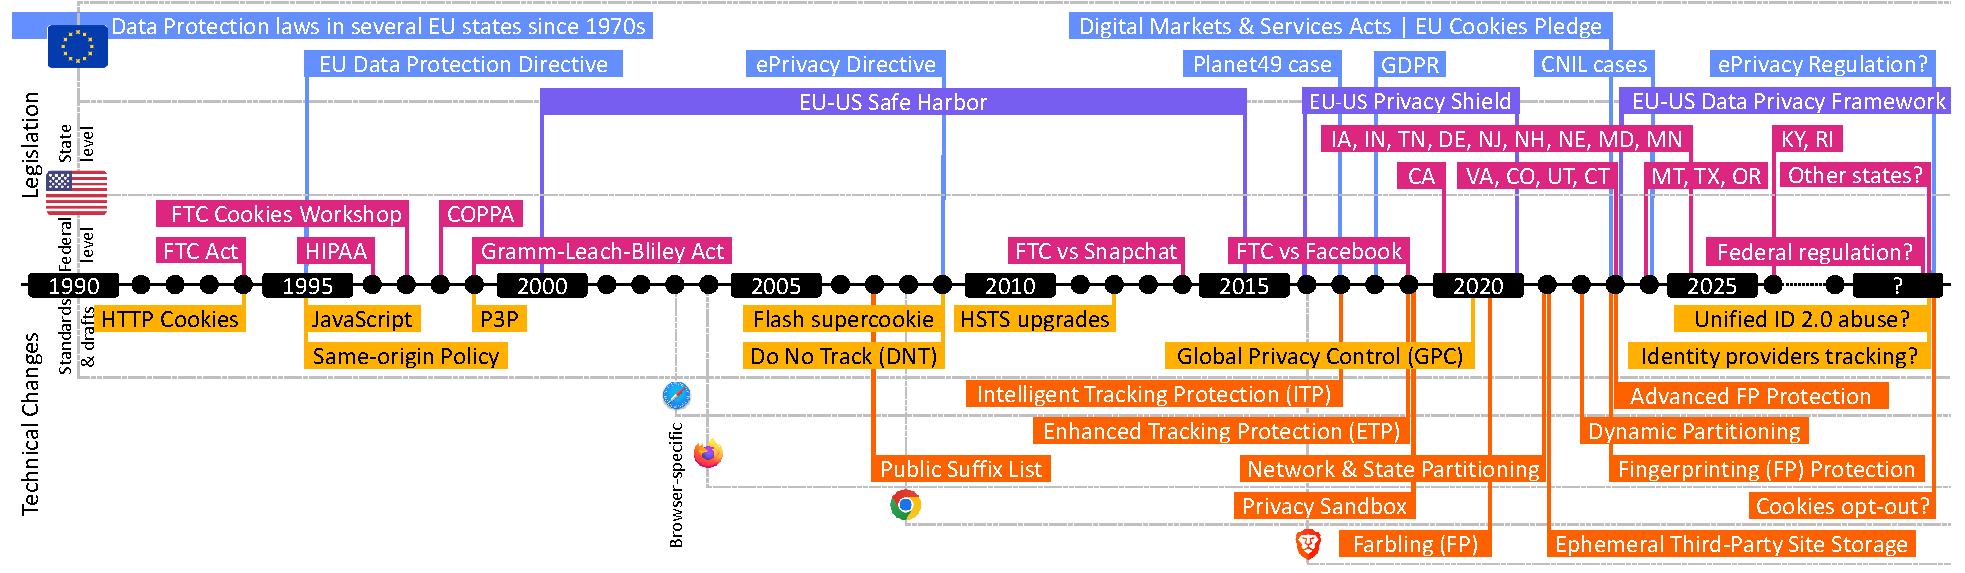
\includegraphics[width=\textwidth]{figures/timeline.pdf}
    \caption{Timeline of major technical and browser-specific changes with regulation overview in the EU and US.}
    \label{fig:timeline}
\end{figure*}

%%
Next, we describe the enactment and evolution of privacy regulations over the years, while many countries worldwide have their own data protection laws~\cite{cnilDataProtectionWorld}, we narrow down our focus on the US and the EU. An overview of technical and regulatory changes is provided in \autoref{fig:timeline}.
%%
\subsection{Regulatory Actions in the US}
\label{sec:us-regulations}

%%
In the US, states enact their own privacy legislation and only a few narrow privacy laws exist at the federal level, notably; the Children’s Online Privacy Protection Act (COPPA)~\cite{ChildrensOnlinePrivacy2013}, the Health Insurance Portability and Accountability Act (HIPAA)~\cite{rightsocrHIPAAPrivacyRule2008}, and the Gramm–Leach–Bliley Act~\cite{GrammLeachBlileyAct2013} about children’s personal, protected health, and personal financial information, respectively. Thus, apart from mandatory provisions, the notice and choice principle---generally implemented via privacy policies (required as mandatory on websites for the very first time by CalOPPA in 2003~\cite{CaliforniaCodeBPC2003})---governs what a recipient of personal information can do with it~\cite{zimmeckInformationPrivacyLaw2013}.

Schaub et al., systematically surveyed this principle~\cite{schaubDesignSpaceEffective2015} and found that notice and choice suffer from a lack of regulatory enforcement~\cite{cranorNecessaryNotSufficient2012}, vagueness and ambiguity of notices~\cite{reidenbergAmbiguityPrivacyPolicies2016}, unusable choice implementations~\cite{habibItsScavengerHunt2020}, and nudging and inconvenience factors~\cite{oconnorUnclearInconspicuousRight2021}. 


Under its jurisdiction, the FTC can consider privacy policies that misrepresent a business's data handling practices as unfair or deceptive, affecting commerce per 15 U.S.C. §45(a)(1)~\cite{unitedstates:congress:houseofrepresentatives:officeofthelawrevisioncounselUnfairMethodsCompetition2023}, and has done so in the past; bringing charges against Snapchat for transmitting geolocation information from its Android users in contradiction to its privacy policy~\cite{ftcSnapchatSettlesFTC2014} or fining Facebook \$5 billion for privacy violations related to the Cambridge Analytica scandal~\cite{FTCImposes52019}. With such enforcement actions over the last few decades, the FTC has effectively created a body of common law of privacy~\cite{soloveFTCNewCommon2013}.  

Similarly, state attorneys general also increased their regulatory activity based on new privacy state laws: California passed the CCPA in 2020 and CPRA in 2023, soon followed by other states as depicted in~\autoref{fig:timeline}: in 2023 by Virginia, Colorado, Utah, and Connecticut, in 2024 by Montana, Texas, and Oregon, all joined in 2025 by nine other states (Iowa, Indiana, Tennessee, Delaware, New Jersey, New Hampshire, Nebraska, Maryland, and Minnesota), and soon in 2026 by at least Kentucky and Rhode Island. 
%
Overall, the systematization and enforcement of privacy laws in the US (and elsewhere) is advancing, though recent changes to the CCPA via the CPRA may negatively impact the usability, scope, and visibility of the right to opt-out of sale~\cite{charatanTwoStepsForward2024}.

%%
\subsection{Regulatory Actions in the EU}
\label{sec:eu-regulations}


%%
In the EU, the first data protection laws were established in several states in late 1970s~\cite{LoiNdeg78171978,GermanDP-1977,NorwayDP-1978}, followed by the EU Data Protection Directive in 1995~\cite{Directive199546EC}, and the General Data Protection Regulation (GDPR) applicable directly to all EU member states in 2018~\cite{Regulation2016679}.  
%
Personal data transfers from the EU to the US are currently regulated by the EU–US Data Privacy Framework~\cite{EU-US-DP-2023} that replaced the EU-US Privacy Shield from 2016~\cite{PrivacyShield-2016} and invalidated in 2020~\cite{Schrems-II}---which itself had replaced the EU-US Safe Harbor from 2000~\cite{SafeHarbor-2000} 
invalidated in 2015~\cite{Schrems-I}.

%
The ePrivacy Directive (2002, amended in 2009) requires in its Article 5(3) a valid user’s consent before \textit{``storing of information, or the gaining of access to information already stored, in the terminal equipment’’}~\cite{Directive2002582002,Directive20091362009}. The GDPR re-defined this notion of valid consent by setting higher-level legal requirements~\cite{santosAreCookieBanners2020}. As efforts to update the ePrivacy Directive into an ePrivacy Regulation---which could introduce stronger and simpler rules on tracking technologies and consent---have not reached a consensus so far~\cite{europeancommissionProposalEPrivacyRegulation2024}, EU regulators continuously update their national laws and compliance guidelines to further interpret and implement the ePrivacy Directive~\cite{Bielova2024-zr}.

Therefore, over the years, EU regulators have interpreted Article 5(3) in different ways to (a) require as early as 2009 the need for consent before cookies are set, read, or sent to third-parties, but also (b) establish that consent is not required for all tracking technologies if their use is ``strictly necessary’’ (for instance for load balancing) or are needed for ``enabling the communication’’, and (c) broaden its coverage to various types of devices (such as mobile and IoT) and technologies (tracking pixels, identifier sharing in URLs)~\cite{Guidelines22023}. 

On the compliance side, EU regulators have been actively investigating tracking technologies, consent, and malpractices. In the Planet49 case, the highest court in the EU (CJEU) established legal precedent by declaring pre-ticked boxes in consent design interfaces illegal~\cite{CJEUC67317}. Similarly the French Data Protection Authority found that consent banners must offer a reject option on the first layer~\cite{ClosureInjunctionIssued2023,CNILFranceSAN2021024}, and companies have been fined for setting cookies prior to consent~\cite{CNILFranceSAN2020012,DeliberationSAN20200127}. For more, we refer readers to the GDPRhub wiki maintained by the Noyb NGO that inventories all EU decisions regarding GDPR~\cite{GDPRhub}.

In recent years, the EU Commission’s Cookie Pledge tried to establish simpler rules for consent~\cite{europeancommissionCookiePledgeEuropean2023}, and new EU laws, such as the Digital Markets Act~\cite{RegulationEU20222022} and Digital Services Act~\cite{RegulationEU20222022a} have set up additional rules on valid consent for the major companies (defined as \textit{``gatekeepers’’}) as well as new requirements for dark patterns and advertising on online platforms, respectively.

%%
\subsection{Policy-oriented Solutions}
\label{sec:policy-solutions}

%%
In order to technically implement an opt out right and consent, several attempts have been made at designing privacy preference signals that would allow users to communicate their data processing choices to online services. However, the adoption and enforcement of such signals by both senders and recipients is an unresolved coordination problem~\cite{hilsPrivacyPreferenceSignals2021}.

\paragraph{The Platform for Privacy Preferences Project (P3P)}~\cite{reaglePlatformPrivacyPreferences1999,cranorPlatformPrivacyPreferences2002,cranorPlatformPrivacyPreferences2006} enabled websites to communicate their privacy practices to users in a standardized and fine-grained format. Nonetheless, its utility was limited by the low number of sites that (a) were adopting it~\cite{cranorUseP3PUser2002} and (b) actually implementing it correctly~\cite{cranorAnalysisP3PDeployment2003} without (c) misleading users~\cite{leonTokenAttemptMisrepresentation2010}. Advanced Data Protection Control~\cite{sustainablecomputinglabAdvancedDataProtection2022} applies a P3P-like approach to the GDPR, though, similar to P3P, exposes a large fingerprinting surface exploitable by probabilistic trackers (see \autoref{sec:stateless-tracking}).


\paragraph{Do Not Track (DNT)}~\cite{fieldingTrackingPreferenceExpression2019} was developed from 2009 as a binary signal for users to express tracking opt out. However, DNT adoption remains low as the California Online Privacy Protection Act, on which DNT is based, only requires online services to say whether or not they respect it~\cite{CaliforniaCodeBPC2003}. Recently, a decision of the Landgericht Berlin---forbidding LinkedIn from ignoring DNT signals and users' decision through them to opt-out from tracking~\cite{CourtProhibitsLinkedins2023}---revitalized DNT. 

\paragraph{Global Privacy Control (GPC)}~\cite{zimmeckGlobalPrivacyControl2024} can be viewed as a successor to DNT. While people find GPC useful and usable, adoption is slow~\cite{zimmeckUsabilityEnforceabilityGlobal2023,zimmeckGeneralizableActivePrivacy2024}, despite GPC compliance being required in California since January 2021~\cite{archive-attorneygeneralbecerra[@agbecerra]CCPARequiresBusinesses2021}---where Sephora was charged for not respecting GPC opt out choices (5.0)~\cite{bontaAttorneyGeneralBonta2022}---and Colorado since July 2024~\cite{coloradodepartmentoflawUniversalOptOutShortlist2024}. Note that even though websites may offer other implementations to their users such as opt-out links, these regulations still ask website publishers to equally respect GPC.
Whether GPC can be applicable in the EU within ePrivacy and GDPR context, is still an open discussion~\cite{berjonGPCGDPR2021}. GPC can also be used to generalize an opt out choice from one site towards a set of others where laws do not allow GPC to be turned on by default~\cite{zimmeckGeneralizableActivePrivacy2024}.

Policy-oriented protocols and frameworks remain in early stages, as evidenced by the Data Rights Protocol~\cite{consumerreportsDataRightsProtocol2024} and industry consent frameworks~\cite{iabtechlabGlobalPrivacyPlatform2024}. It also appears unclear how opt out functionalities elsewhere (such as with mobile applications) align with the opt out right.


